%Note di Ingegneria del Software
%Sommario: Fine dei diagrammi di attività, Diagrammi di sequenza, inizio dei design pattern

\cornell[Parte mancata]{Causa Ritardo}{Fine dei diagrammi di attività}

\cornell{Diagrammi di sequenza}{Descrivono la collaborazione di un gruppo di oggetti che devono implementare collettivamente un comportamento\\
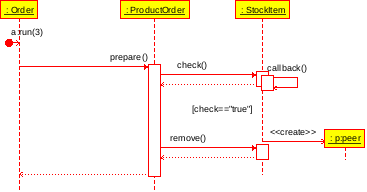
\includegraphics[scale=0.7]{images/54.png}}

\cornell{Diagramma delle classi corrispondente (Di Order, ProductOrder e StockItem)}{
        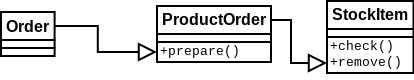
\includegraphics[scale=0.5]{images/55.png}
}

\cornell{Messaggi}{Dati e operazioni scambiati tra i partecipanti \begin{itemize}
\item Chiamate a metodi di oggetti
\item Messaggio trovato
\end{itemize}}

\cornell{Messaggi e Dipendenze}{Gli attori possono inviarsi messaggi \textbf{solo se} tra loro vi è qualche dipendenza}

\cornell{Tipi di Segnali/Messaggi}{ 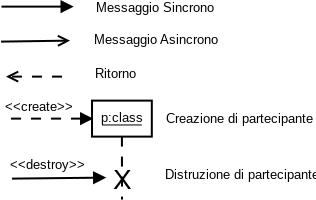
\includegraphics[scale=0.7]{images/56.png} }

\cornell{Passaggio di dati e parametri}{Non vi è alcuna tecnica standard per il passaggio di parametri, solitamente si usano:\\
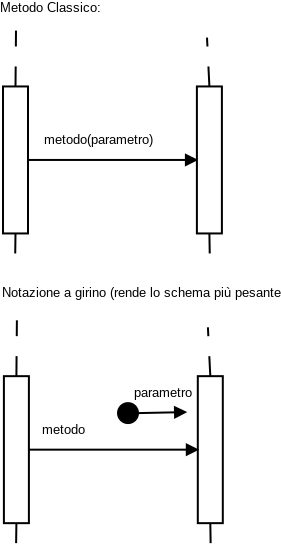
\includegraphics[scale=0.5]{images/57.png}}

\cornell{Cicli e condizioni}{Il diagramma di sequenza non sarebbe il più adatto per descrivere cicli e condizioni, ma si possono usare "frame di interazione", questi purtroppo tolgono il concetto di tempo che scorre dall'alto in basso del diagramma (cosa importante).\\
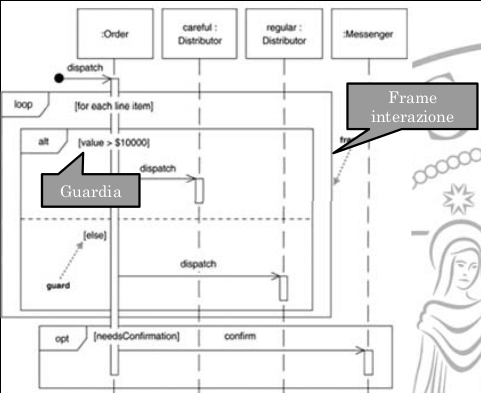
\includegraphics[scale=0.5]{images/58.png}}

\cornell{Diagrammi centralizzati vs Diagrammi distribuiti}{ \begin{description}
\item [Diagrammi Centralizzati] Un attore controlla tutto il flusso di esecuzione, il che porta un oggetto ad avere troppe responsabilità; quindi in caso di cambiamento dei requisiti, questo oggetto dovrà probabilmente cambiare (Paradigma Procedurale)
\item [Diagrammi Distribuiti] Vi è un "rincorrersi di messaggi" tra più oggetti diversi (Paradigma Object Oriented)
\end{description} }

\cornell{Design Pattern Strutturali}{Affrontano problemi riguardanti composizione di classi ed oggetti, consentono il riuso e sfruttano ereditarietà ed aggregazione.}

\cornell{Adapter}{Converte l'interfaccia di una classe in un'altra.\\
Perchè? Perchè spesso i toolkit non sono riusabili (ad esempio librerie provenienti dall'esterno).\\
Questo pattern permette il riuso di una classe esistente che però non è conforme all'interfaccia target.\\
Permette la creazione di classi riusabili, anche con classi non ancora viste.\\
Da usare in caso non sia possibile riadattare l'interfaccia tramite l'ereditarietà (Vedi Object adapter)}
